\documentclass{article}

\usepackage[preprint]{neurips_2025}
\usepackage[utf8]{inputenc}
\usepackage[T1]{fontenc}
\usepackage{hyperref}
\usepackage{url}
\usepackage{booktabs}
\usepackage{amsfonts}
\usepackage{amsmath}
\usepackage{graphicx}
\usepackage{xcolor}
\usepackage{microtype}
\usepackage{multirow}
\usepackage{array}
\usepackage{caption}
\usepackage{subcaption}

\title{Multimodal CAD Code Generation from Images and Point Clouds}

\author{
  Nicholas Sung \\
  Department of Mechanical Engineering \\
  Massachusetts Institute of Technology \\
  \texttt{nicksung@mit.edu} \\
  \url{https://github.com/nicksungg/trimodal-cad}
  \and
  Anna C. Doris \\
  Department of Mechanical Engineering \\
  Massachusetts Institute of Technology \\
  \texttt{adoris@mit.edu}
}

\begin{document}

\maketitle

\begin{abstract}
Editable CAD reconstruction is a harder target than ordinary 3D shape generation because the output must be executable, parametric, and useful to an engineer after generation. Recent image-conditioned systems such as CAD-Coder show that vision-language models can generate valid CadQuery programs from rendered inputs, while point-cloud systems such as CAD-Recode show that explicit 3D geometry can improve reconstruction fidelity. This project studies a lightweight multimodal extension that conditions a language model on both rendered views and point clouds by projecting frozen modality features into the decoder embedding space. Due to compute and time constraints, the experimental scope consists of two baselines, CAD-Coder and CAD-Recode, plus the single model we implemented: a projection-only multimodal CAD generator in which only small modality projectors are tuned while the image encoder, point-cloud encoder, and language-model backbone remain frozen. The resulting study is therefore framed as a controlled diagnostic result: can inexpensive prefix-token multimodal alignment make a frozen CAD generator competitive with image-only and point-cloud-only baselines? Projection-only tuning is attractive because it is cheap and stable, but it may underfit the cross-modal alignment needed for precise CAD program synthesis, especially for occluded features, small holes, and high-face-count parts. The report presents the model, benchmark protocol, quantitative results, and an error-analysis plan focused on executability, geometric overlap, and failure modes.
\end{abstract}

\section{Introduction}

Computer-aided design (CAD) is central to engineering practice, from consumer products to aerospace and manufacturing. Yet CAD modeling remains a slow, expertise-heavy process: prior work on engineering cost estimation reports that experienced aerospace engineers can spend weeks modeling a single complex component~\cite{roy2001quantitative}. Automating even part of this workflow could reduce repetitive drafting effort, accelerate design iteration, and make parametric modeling more accessible to non-expert users. For engineering applications, however, the target representation matters. Meshes, voxels, and point clouds can capture appearance or surface geometry, but they do not preserve the editable construction logic that designers use in practice. CAD programs, such as CadQuery Python scripts, encode sketches, constraints, extrusions, booleans, fillets, and other feature operations, making them a more useful output for downstream editing and manufacturing.

The research challenge is that editable CAD generation requires both geometric understanding and symbolic program synthesis. Vision-language models have recently shown that rendered images can condition executable CAD code generation~\cite{cadcoder}, and point-cloud-conditioned systems show that explicit 3D geometry can improve reconstruction fidelity~\cite{cadrecode}. These two modalities are complementary: images provide semantic cues, silhouettes, and sharp visual boundaries, while point clouds provide an occlusion-free spatial scaffold. However, prior image-only methods must infer hidden geometry such as rear faces, internal cuts, and through-holes from incomplete projections. Prior point-cloud-only methods reduce this ambiguity but may lack the visual and semantic context available in rendered views. Existing multimodal CAD systems often combine modalities through simple projection and token concatenation~\cite{cadmllm}, placing the burden of cross-modal alignment on the language model rather than explicitly studying whether lightweight alignment is sufficient for CAD code generation.

In this paper, we study a practical multimodal CAD code generation model that conditions an autoregressive language model on both multi-view images and point clouds. The model uses frozen image and point-cloud encoders and trains only lightweight projectors that map both modalities into the language-model embedding space before decoding CadQuery code. This design intentionally tests a conservative question: can cheap prefix-token multimodal alignment make a frozen CAD generator competitive with strong unimodal baselines? We compare against CAD-Coder as the image-only baseline and CAD-Recode as the point-cloud-only baseline. Figure~\ref{fig:overview} summarizes the proposed pipeline, in which rendered views and explicit 3D samples are fused as prefix tokens before CAD code generation.

\begin{figure}[t]
  \centering
  \includegraphics[width=\linewidth]{figures/summary_placeholder_v2.png}
  \caption{Overview of the proposed multimodal CAD generation pipeline.}
  \label{fig:overview}
\end{figure}

\section{Related Work}

\paragraph{Editable CAD representations and datasets.}
Most 3D generative modeling work produces static geometry, but engineering CAD workflows require editable feature histories. DeepCAD framed CAD generation as a sequence modeling problem over sketch-and-extrude operations and released a dataset of construction sequences~\cite{wu2021deepcad}. SkexGen further disentangles sketch and extrusion representations for autoregressive CAD construction~\cite{skexgen}. Point2CAD approaches reverse engineering from point clouds through a hybrid analytic-neural pipeline for CAD surface reconstruction~\cite{point2cad}. Dataset work has also shaped the field: ABC provides a large collection of CAD models with parametric surfaces~\cite{koch2019abc}, MCB focuses on categorized mechanical components~\cite{sangpil2020large}, Objaverse broadens evaluation to diverse 3D assets~\cite{deitke2023objaverse}, CADBench unifies multimodal CAD-program evaluation across datasets and input modalities~\cite{cadbench}, and CADEvolve generates large-scale executable CadQuery programs through program evolution~\cite{elistratov2026cadevolve}. Our work follows the editable-program direction, using CadQuery code rather than static mesh reconstruction as the target representation.

\paragraph{Point-cloud and multimodal representation learning.}
Point clouds are unordered sets, so early 3D networks focused on permutation-invariant and local geometric processing. PointNet introduced shared pointwise processing with symmetric aggregation~\cite{qi2017pointnet}; PointNet++ added hierarchical local neighborhoods~\cite{qi2017pointnet++}; and PointCNN learned transformations for local point convolution~\cite{li2018pointcnn}. More recent self-supervised methods such as Point-BERT, Point-MAE, and PCP-MAE learn stronger 3D features through masked point modeling and reconstruction~\cite{yu2022point,pang2023masked,zhang2024pcp}. A separate line aligns 3D with other modalities: CLIP established large-scale image-text alignment~\cite{radford2021clip}, while CrossPoint, PointCLIP, and Michelangelo extend alignment to image-point or shape-image-text spaces~\cite{afham2022crosspoint,zhang2022pointclip,zhao2023michelangelo}. These representations are strong for recognition, retrieval, and shape generation, but they are not directly optimized for the operation-level decisions required by CAD program synthesis.

\paragraph{Image-conditioned CAD generation.}
Several systems reconstruct editable CAD from visual inputs. GenCAD learns a joint latent space between CAD programs and rendered images, then uses a diffusion prior to map image latents into CAD program latents~\cite{alam2024gencad}. CAD-Coder instead fine-tunes a vision-language model to generate executable CadQuery Python directly from image input, benefiting from pretrained vision-language and code knowledge~\cite{cadcoder}. Img2CAD uses VLM-assisted conditional factorization for reverse engineering CAD models from images~\cite{img2cad}, and CADCrafter studies CAD generation from unconstrained images~\cite{cadcrafter}. These methods motivate image-conditioned CAD code generation, but image-only reconstruction remains underdetermined whenever critical geometry is occluded or visually ambiguous.

\paragraph{Point-cloud and multimodal CAD generation.}
To reduce image ambiguity, recent work conditions CAD generation on explicit 3D geometry. CAD-Recode maps point-cloud tokens to executable CAD code using a lightweight projector and an LLM decoder~\cite{cadrecode,rukhovich2025cad}. Cadrille extends this direction with multimodal reconstruction and online reinforcement learning~\cite{kolodiazhnyi2025cadrille}, echoing broader work such as CodeRL that uses execution feedback to improve program generation~\cite{le2022coderl}. CAD-MLLM unifies text, image, and point inputs by projecting modality-specific features, including DINOv2 image features~\cite{oquab2023dinov2} and Michelangelo-style 3D features, into an LLM for CAD generation~\cite{cadmllm}. These works show the promise of multimodal CAD generation, but many current systems still rely on frozen encoders, learned projectors, and early token concatenation.

\paragraph{How our work differs.}
Our project is not the first to use images, point clouds, or language models for CAD generation. Instead, it isolates a practical question left open by the above literature: how much benefit can be obtained from the simplest multimodal fusion strategy when most of the system is frozen? Compared with CAD-Coder, we add explicit 3D point-cloud evidence; compared with CAD-Recode, we add rendered visual context; compared with CAD-MLLM and Cadrille, we do not claim a full multimodal foundation model or reward-optimized system. Our contribution is a controlled evaluation of projection-only prefix-token fusion for CadQuery generation against image-only and point-cloud-only baselines, clarifying whether future work should invest in deeper adapter tuning, multi-layer geometric injection, or CAD-specific reward optimization.

\section{Problem Statement}

Let an object be represented by a multimodal input $X=(I,P)$, where $I=\{I_1,\dots,I_V\}$ is a set of $V$ rendered views and $P=\{p_1,\dots,p_N\}\in\mathbb{R}^{N\times3}$ is a sampled point cloud. The desired output is a CadQuery Python program $S=(s_1,\dots,s_T)$, where each token $s_t$ belongs to the decoder vocabulary. The generated program should satisfy three constraints: syntactic validity as Python, executable validity under CadQuery, and geometric similarity to the target object.

The supervised learning objective is the conditional negative log-likelihood
\begin{equation}
\mathcal{L}_{\mathrm{NLL}}(\theta)
=-\sum_{t=1}^{T}\log p_{\theta}(s_t \mid s_{<t}, I, P),
\end{equation}
where the conditioning inputs are only the rendered image view and point cloud. In our proposed model, most parameters are frozen. If $\phi_I$ is the image encoder, $\phi_P$ is the point-cloud encoder, and $D$ is the language-model decoder, then only the modality projectors $g_I$ and $g_P$ are optimized:
\begin{equation}
\theta_{\mathrm{train}}=\{g_I,g_P\}, \qquad
\theta_{\mathrm{frozen}}=\{\phi_I,\phi_P,D\}.
\end{equation}
The research question is whether this restricted trainable parameter set is sufficient to align visual and geometric features with CAD-code generation decisions.

\section{Proposed Method}

\paragraph{Input construction.}
Each CAD example is represented by aligned code, rendered images, and a point cloud. We treat each rendered view as a separate image-conditioned training row paired with the same point cloud and CadQuery target program, giving supervision from multiple viewpoints without changing the target code. Images are converted to RGB and processed at the input resolution expected by the vision backbone. The point cloud is represented as an unordered set of 3D coordinates and reduced to 256 points using deterministic farthest-point sampling, which preserves broad surface coverage while keeping the multimodal prefix length manageable.

\paragraph{Frozen image branch.}
The image branch uses a frozen DINOv2-base vision transformer to extract robust visual features~\cite{oquab2023dinov2}. We keep the full last-layer visual token sequence rather than reducing the view to a single global vector, since local patch tokens can preserve evidence for small holes, protrusions, and silhouette changes. These visual tokens are mapped into the language-model hidden dimension by a trainable two-layer GELU MLP projector:
\begin{equation}
Q_I = g_I(\phi_I(I)).
\end{equation}
Because $\phi_I$ is frozen, the image branch can adapt only by learning how to express existing DINOv2 features as prefix tokens that the decoder can attend to.

\paragraph{Frozen point-cloud branch.}
The point branch follows the CAD-Recode motivation of translating explicit 3D evidence into language-model conditioning tokens~\cite{cadrecode}. Each sampled point is encoded with a frozen Fourier feature point encoder: the raw $(x,y,z)$ coordinate is expanded with sinusoidal features over eight frequency bands and then projected to the decoder hidden size. This produces a sequence of geometric tokens, one per sampled point. A second trainable two-layer GELU MLP then maps those frozen geometric features into the same prefix-token space as the image branch:
\begin{equation}
Q_P = g_P(\phi_P(P)).
\end{equation}
This design gives the model direct access to 3D spatial evidence while still limiting trainable capacity to the modality-alignment layers.

\paragraph{Multimodal token fusion.}
The projected image tokens and point-cloud tokens are concatenated before autoregressive decoding:
\begin{equation}
Z_0 = [Q_I; Q_P],
\end{equation}
where $Z_0$ is the multimodal prefix supplied to the decoder. The decoder then predicts the CadQuery program token by token:
\begin{equation}
p_{\theta}(S\mid I,P)=\prod_{t=1}^{T}p_{\theta}(s_t\mid s_{<t},Z_0).
\end{equation}
This approach keeps the implementation simple and avoids modifying transformer internals. The tradeoff is that all cross-modal interaction must be learned through the projectors and the frozen decoder's existing attention layers.

\paragraph{Decoder and training objective.}
The decoder is a frozen Qwen2-1.5B causal language model. The multimodal prefix is prepended directly to the CadQuery token sequence through the decoder input embeddings. During training, attention is enabled over both the prefix and code tokens, but the prefix positions are assigned an ignore label, so the loss is computed only on the target CadQuery program tokens. This preserves the usual autoregressive code-generation objective while allowing every generated token to attend to image and point-cloud context.

\paragraph{Optimization.}
The completed training run uses a projector-warmup stage: DINOv2, the Fourier point encoder, and Qwen2 remain frozen, while the two modality projectors are optimized. The resulting trainable set contains approximately 8.26M parameters, a small fraction of the full model. We train with AdamW at a learning rate of $2\times10^{-4}$, batch size 4, maximum code length 1024 tokens, gradient clipping at norm 1.0, and checkpointed multi-GPU training. Training took approximately three weeks on two NVIDIA H100 GPUs. The checkpoint used for downstream evaluation was obtained after a long resumed run of the projector-only stage, reaching 1.23M optimization steps. At inference time, the model directly conditions on the image and point cloud and autoregressively decodes up to 256 new tokens, after which the generated program is executed and exported through the CAD kernel for feasibility and geometry evaluation.

\paragraph{Models compared.}
The experimental comparison contains two baselines and one proposed model:
\begin{itemize}
  \item \textbf{CAD-Coder baseline.} Image-conditioned CadQuery generation using the CAD-Coder setup. This establishes the vision-only reference point.
  \item \textbf{CAD-Recode baseline.} Point-cloud-conditioned CAD code generation. This establishes the geometry-only reference point.
  \item \textbf{Ours: projection-only multimodal model.} Multimodal image and point-cloud conditioning with frozen encoders and frozen LLM backbone. Only the final modality projectors into the decoder embedding space are trained.
\end{itemize}
Unrun variants such as adapter fine-tuning, full LLM fine-tuning, or reinforcement learning are treated as future work, not as completed experiments.

\section{Experimental Methodology}

\paragraph{Training data.}
The training setup is based on CADEvolve, a large executable CadQuery corpus paired with rendered geometry~\cite{elistratov2026cadevolve}. We train from 923{,}104 CAD samples. Each sample contains a CadQuery script, eight rendered views, and a 256-point point cloud:
\[
(\mathrm{code}, I_1,\dots,I_8, P).
\]
During training, each rendered view is paired with the same point cloud and target script, yielding 7.38M individual image--point-cloud pairs (7{,}384{,}832 total). This pairing is important because both modalities supervise the same target program rather than separate shape labels.

\paragraph{Evaluation benchmarks and splits.}
To rigorously assess syntactic validity and geometric fidelity across diverse domains, we divide evaluation into five distinct test environments:
\begin{itemize}
    \item \textbf{DeepCAD}~\cite{wu2021deepcad} (3{,}000 samples; 1{,}000 each for Easy, Medium, and Hard): Human-designed models for evaluating standard CAD adherence.
    \item \textbf{ABC-Simple}~\cite{koch2019abc} (3{,}000 samples; 1{,}000 each for Easy, Medium, and Hard): Samples containing primarily sketch-and-extrude style operations.
    \item \textbf{ABC-Complex}~\cite{koch2019abc} (3{,}000 samples; 1{,}000 each for Easy, Medium, and Hard): Samples with more complex operations such as fillet, revolve, chamfer, and compound topology.
    \item \textbf{Mechanical Components Benchmark (MCB)}~\cite{sangpil2020large} (3{,}000 samples): Mechanical Components Benchmark for engineering-focused evaluation.
    \item \textbf{Objaverse}~\cite{deitke2023objaverse} (3{,}000 samples): Zero-shot transfer to generalized, in-the-wild object geometries.
\end{itemize}
For DeepCAD, ABC-Simple, and ABC-Complex, samples are partitioned evenly across complexity bins and selected to maximize diversity from one another in latent space, so that each subset covers a broad range of geometries rather than concentrating on highly similar examples. Following the CADBench protocol~\cite{cadbench}, Easy, Medium, and Hard are treated as \emph{complexity tiers} rather than subjective labels. For STEP-based families, complexity is measured by B-rep face count, which is consistent across STEP data, reflects the number of surfaces defining a part, and correlates with expert-perceived modeling difficulty. CADBench first splits the logarithmic face-count range within each family, then adjusts thresholds so each tier contains at least 1{,}000 samples; the resulting thresholds are dataset-specific rather than universal. Mesh-based families such as MCB and Objaverse are not split by mesh face count because tessellation density is not a reliable proxy for CAD modeling complexity.

\paragraph{Metrics.}
We report two primary metrics. \textbf{STEP feasibility} measures the percentage of generated programs that execute and export to a valid STEP file. This captures practical CAD usability. \textbf{IoU} measures geometric overlap between predicted and target shapes. Together, these metrics separate code validity from geometric accuracy: a model can generate executable code that produces the wrong object, or geometrically plausible code that fails under the CAD kernel.

This two-metric view is intentionally minimal, but it should be interpreted in the context of broader CADBench-style evaluation~\cite{cadbench}. CADBench argues that editable CAD program quality spans at least three axes: geometric fidelity, executability, and program compactness. Volumetric IoU captures coarse occupancy agreement, but it can miss small surface features such as shallow slots, fillets, and holes that occupy little volume. Chamfer distance and surface IoU are more sensitive to local boundary alignment, while token count and operation count help distinguish concise editable programs from bloated scripts that happen to render a similar solid. We focus on feasibility and IoU because they are the most available metrics for the completed runs, but the qualitative analysis below should be read as compensating for this limitation: it inspects where high feasibility hides missing fine-grained CAD structure.

\paragraph{Metric caveats.}
STEP feasibility is necessary but not sufficient. A generated script can execute, export, and produce a valid solid while still using the wrong construction sequence or the wrong dimensions. Conversely, IoU is a useful global geometry score but does not measure editability, semantic feature correspondence, or whether the predicted program uses the same design intent as the target. In engineering use, two shapes with similar volume overlap can differ substantially in whether a user can change a radius, adjust a slot, suppress a fillet, or reuse the model in an assembly. For this reason, the results are interpreted as a diagnostic of first-stage multimodal alignment rather than a final claim about deployable CAD automation.

\paragraph{Implementation details.}
Our multimodal model uses Qwen2-1.5B as the frozen causal decoder, DINOv2-base as the frozen image encoder, and a frozen Fourier point encoder initialized from the point-cloud branch. The training manifest contains 7.38M image-view rows (7{,}384{,}832 total) expanded from 923{,}104 CAD samples, with each row pairing one rendered view, one 256-point sample, and the corresponding CadQuery program. The two trainable MLP projectors map image and point features into the 1536-dimensional decoder embedding space. This setup is intentionally parameter efficient: the encoders and decoder provide reusable representations, while optimization is restricted to the cross-modal alignment interface.

\begin{figure}[t]
  \centering
  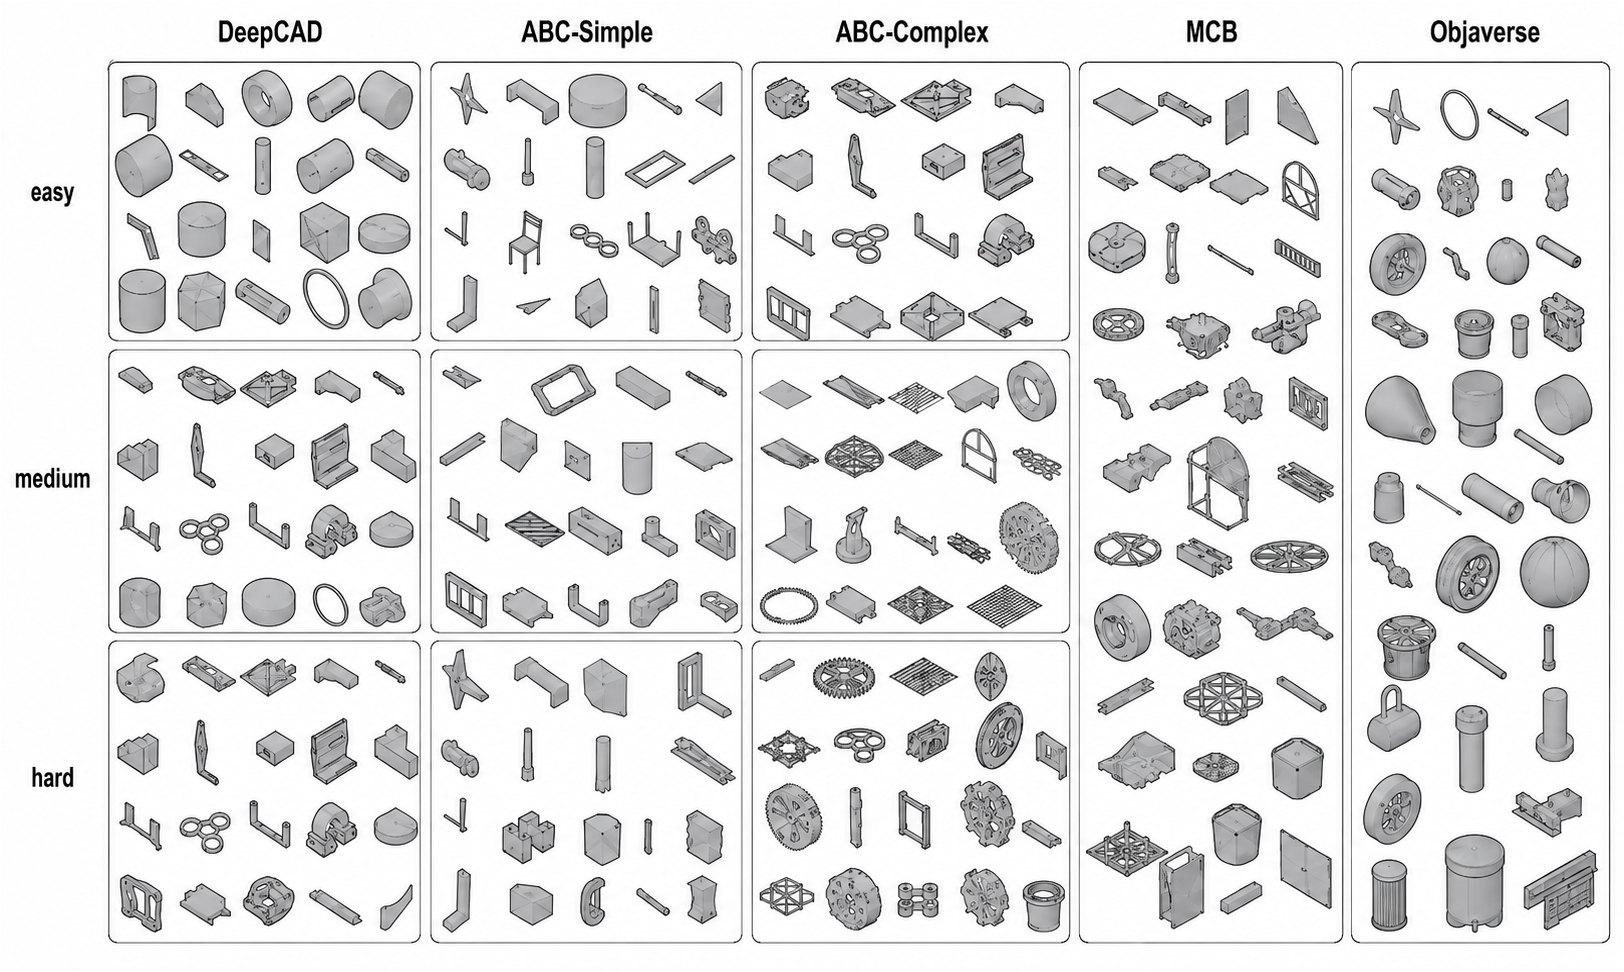
\includegraphics[width=\linewidth]{figures/cad_bench.png}
  \caption{\textbf{CADBench-style benchmark visualization.} The evaluation suite covers DeepCAD, ABC-Simple, ABC-Complex, MCB, and Objaverse. STEP-based datasets are stratified into Easy, Medium, and Hard tiers by B-rep face-count complexity, while mesh-based families are evaluated without face-count tiers.}
  \label{fig:cadbench}
\end{figure}

\section{Results and Discussion}

\paragraph{Main quantitative results.}
Table~\ref{tab:main_results} compares the two baselines with our implemented multimodal model. CAD-Coder values are included as the image-only baseline, CAD-Recode values are included as the point-cloud-only baseline, and our projection-only multimodal results are reported across the same benchmark suite.

\begin{table*}[t]
\centering
\caption{Evaluation results. STEP feasibility and IoU are percentages; higher is better. CAD-Coder is the image-only baseline and CAD-Recode is the point-cloud-only baseline.}
\label{tab:main_results}
\resizebox{\textwidth}{!}{
\begin{tabular}{@{}llccccccccccc@{}}
\toprule
\multirow{2}{*}{\textbf{Model}} & \multirow{2}{*}{\textbf{Metric}}
& \multicolumn{3}{c}{\textbf{DeepCAD}}
& \multicolumn{3}{c}{\textbf{ABC-Simple}}
& \multicolumn{3}{c}{\textbf{ABC-Complex}}
& \textbf{MCB}
& \textbf{Objaverse} \\
\cmidrule(lr){3-5} \cmidrule(lr){6-8} \cmidrule(lr){9-11}
&
& \textbf{E} & \textbf{M} & \textbf{H}
& \textbf{E} & \textbf{M} & \textbf{H}
& \textbf{E} & \textbf{M} & \textbf{H}
& \textbf{All}
& \textbf{All} \\
\midrule
\multirow{2}{*}{CAD-Coder (image-only)}
& STEP Feasibility & 96.0 & 96.8 & 92.4 & 99.6 & 96.6 & 95.8 & 92.4 & 76.0 & 83.4 & 99.6 & 97.8 \\
& IoU Mean         & 62.8 & 58.3 & 54.0 & 60.2 & 51.0 & 61.6 & 56.5 & 45.5 & 49.6 & 58.5 & 35.4 \\
\midrule
\multirow{2}{*}{CAD-Recode (point-cloud-only)}
& STEP Feasibility & 97.4 & 95.2 & 94.4 & 96.0 & 87.4 & 85.8 & 92.6 & 89.4 & 89.2 & 93.8 & 88.0 \\
& IoU Mean         & 96.3 & 90.1 & 85.8 & 89.2 & 83.1 & 73.4 & 88.5 & 74.1 & 64.3 & 97.5 & 63.5 \\
\midrule
\multirow{2}{*}{Ours (projection-only multimodal)}
& STEP Feasibility & 93.2 & 93.6 & 96.4 & 94.4 & 83.8 & 80.2 & 98.7 & 95.2 & 96.2 & 99.2 & 98.2 \\
& IoU Mean         & 33.0 & 24.6 & 18.3 & 28.5 & 13.1 & 14.7 & 22.1 & 17.9 & 14.8 & 52.0 & 20.0 \\
\bottomrule
\end{tabular}
}
\end{table*}

\paragraph{Result interpretation.}
The projection-only model should be interpreted as a first-stage alignment result rather than a completed multimodal CAD system. Its main positive signal is executability: the model produces feasible STEP files at an average rate of 93.6\%, and 9 of the 11 benchmark settings are above 93\% feasibility. This suggests that the frozen decoder retains useful CadQuery syntax and that the learned multimodal prefix is compatible with executable code generation. In other words, the first-stage adapters are doing the basic job they were meant to do: they can condition the language model without destroying its ability to emit runnable CAD scripts.

The geometric results show the limitation of this stage. Our model's mean IoU is substantially below both CAD-Coder and CAD-Recode on most benchmark splits, even when feasibility is high. This separation between valid code and accurate geometry is expected in programmatic CAD generation: producing syntactically valid CadQuery is a weaker requirement than selecting the right construction planes, sketch profiles, feature dimensions, boolean operations, and repeated structures. The strongest result for our model is on MCB, where IoU reaches 52.0\% with 99.2\% feasibility, but the DeepCAD and ABC trends show that the current projector-only alignment often captures a coarse executable shape while missing the operation-level structure needed for high-overlap reconstruction.

The qualitative trend in Figure~\ref{fig:failure_progression} shows the same pattern at the shape level. For simple low-face-count shapes, the generated CAD model can be almost identical to the target and achieve near-perfect IoU. In medium-complexity cases, the model often preserves the main silhouette but loses refined features such as holes, slots, and small cuts. In hard examples with many surfaces or repeated local features, the model can still emit executable code but collapse to a much simpler primitive-like object, producing low geometric overlap despite passing the STEP feasibility check.

These results are consistent with the broader CAD-code literature. CAD-Coder demonstrates that VLM fine-tuning can strongly preserve executable CadQuery generation from images~\cite{cadcoder}, while CAD-Recode shows that point-cloud conditioning can yield much stronger geometric fidelity when the decoder and point interface are trained for CAD reverse engineering~\cite{cadrecode}. CADEvolve further indicates that moving from supervised warmup to stronger data processing and reward-based optimization can close much of the remaining IoU gap in Image2CAD settings~\cite{elistratov2026cadevolve}. Our first-stage result therefore narrows the diagnosis: feasibility is not the main bottleneck, but geometric grounding and cross-modal program planning remain undertrained.

\paragraph{Comparison across model families.}
The three rows of Table~\ref{tab:main_results} illustrate three different operating regimes. CAD-Coder benefits from image-conditioned code fine-tuning: it is strong at producing runnable CadQuery and often captures visually salient silhouettes, but it is still limited by what can be inferred from rendered views. CAD-Recode benefits from explicit 3D observations and from training the point-to-code pathway for reverse engineering, so it achieves much higher IoU on the CAD-like benchmark families. Our model sits between these ideas architecturally but not yet in performance: it has both image and point inputs, yet freezes most of the machinery that would let these modalities reshape the decoder's CAD-specific planning. The result is a model that inherits enough code prior to remain executable, but not enough geometric adaptation to compete with CAD-Recode's point-conditioned reconstruction fidelity.

This comparison also explains why adding a modality is not automatically beneficial. The image and point-cloud streams enter as prefix tokens, and the frozen decoder must learn to use them through attention patterns that were not originally trained for this exact multimodal CAD setting. If the projectors underfit, the point tokens may provide spatial evidence that is syntactically visible to the decoder but not semantically organized around CAD operations. In that case, the model can learn broad object cues but fail to bind them to construction decisions such as sketch plane selection, profile closure, extrusion depth, boolean ordering, or repeated feature placement.

\paragraph{Interpreting negative results.}
A weak IoU result for our model is therefore still meaningful. Projector-only tuning freezes the representations that must jointly solve geometry perception, cross-modal correspondence, program planning, and Python/CadQuery decoding. Small projection layers can rotate and scale features into the decoder space, but they cannot deeply reshape the modality encoders around CAD-specific concepts such as construction planes, profile loops, boolean operations, or repeated parametric patterns. This can produce a model that attends to broad shape cues while missing the operation-level structure required for accurate CAD code.

\paragraph{Next training stages.}
The natural next step is not to discard the multimodal design, but to continue the staged training plan. Stage 2 should unfreeze a deeper part of the adaptation stack, such as the modality adapters and selected language-model layers, so that image tokens, point tokens, and code tokens can co-adapt around CAD-specific geometry. Stage 3 should add CAD-aware reward optimization after supervised tuning, using rewards for executable code, valid STEP export, single-solid validity, and geometric overlap. This direction is motivated by program-generation work that uses execution feedback to improve functional correctness~\cite{le2022coderl} and by recent CAD systems that optimize reconstruction quality with geometry-aware rewards~\cite{kolodiazhnyi2025cadrille,elistratov2026cadevolve}. Under this framing, the current model is a successful feasibility warmup but an incomplete geometry learner.

\paragraph{Failure categories.}
The final analysis should group generated examples into at least four categories:
\begin{itemize}
  \item \textbf{Execution failures:} Python syntax errors, missing imports, invalid CadQuery calls, non-solid results, or STEP export failures.
  \item \textbf{Topological failures:} missing through-holes, extra cuts, wrong number of repeated features, disconnected solids, or incorrect boolean structure.
  \item \textbf{Dimensional failures:} correct broad topology but wrong aspect ratio, thickness, radius, or relative placement.
  \item \textbf{Representation failures:} code is valid but unnecessarily complex, brittle, or not meaningfully editable.
\end{itemize}
This breakdown is more useful than a single IoU number because different failure types imply different fixes.

\begin{figure}[t]
  \centering
  \begin{subfigure}{0.32\linewidth}
    \centering
    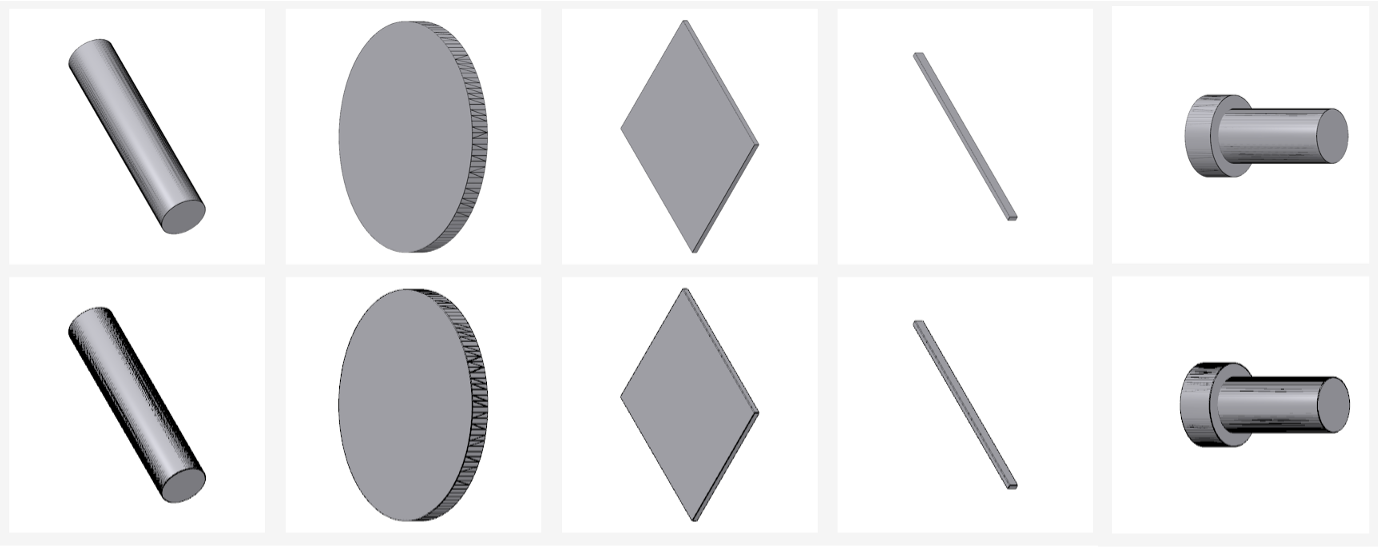
\includegraphics[width=\linewidth]{figures/easy_output.png}
    \caption{Easy}
  \end{subfigure}
  \hfill
  \begin{subfigure}{0.32\linewidth}
    \centering
    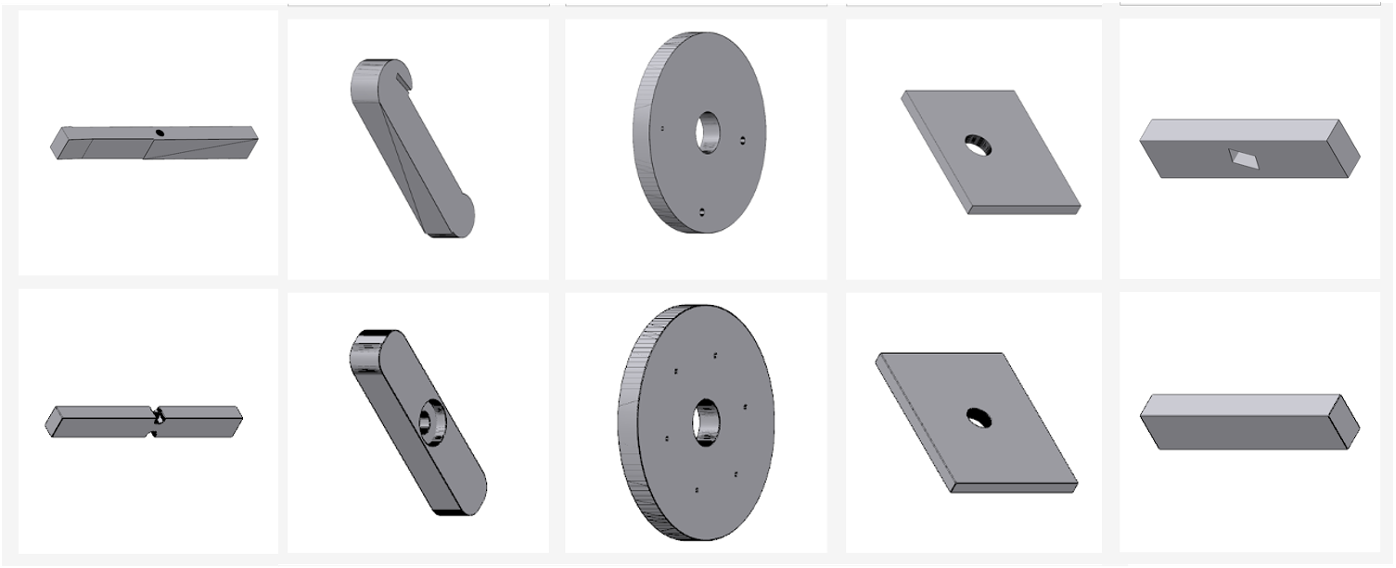
\includegraphics[width=\linewidth]{figures/medium_output.png}
    \caption{Medium}
  \end{subfigure}
  \hfill
  \begin{subfigure}{0.32\linewidth}
    \centering
    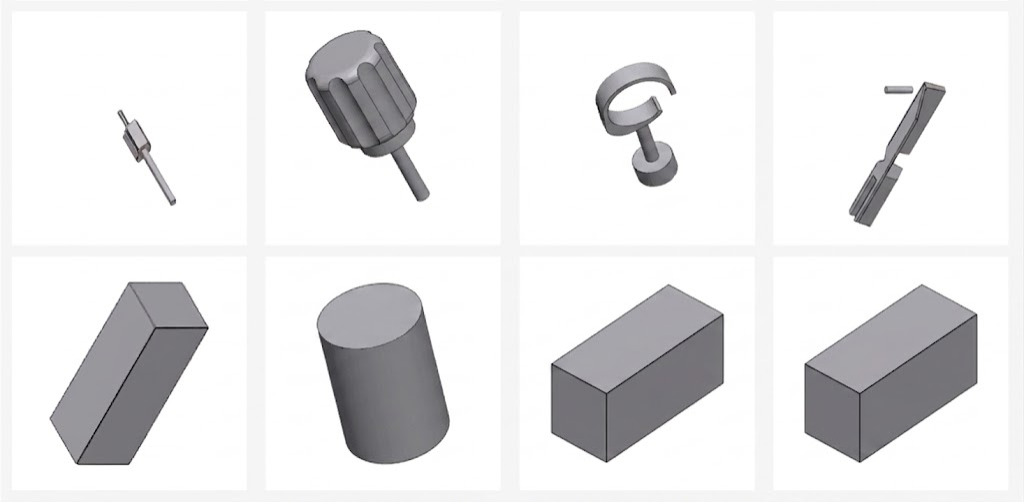
\includegraphics[height=0.40\linewidth,keepaspectratio]{figures/hard_output.png}
    \caption{Hard}
  \end{subfigure}
  \caption{\textbf{Qualitative failure progression.} Easy shapes are often reconstructed almost exactly, medium shapes preserve the main body but miss refined features, and hard shapes with many surfaces can collapse to coarse primitives even when the generated CadQuery remains executable.}
  \label{fig:failure_progression}
\end{figure}

\paragraph{Ablations that remain missing.}
Because we implemented only the projection-only multimodal model, the current evidence cannot determine whether multimodal conditioning is fundamentally limited or whether the projectors were simply too weak. The most important missing ablations are point-only versus image-only within the same codebase, image+point with trainable adapters, and image+point with partial LLM fine-tuning. These comparisons would separate modality value from training-capacity limitations.

\paragraph{Threats to validity.}
Several factors limit the conclusions that can be drawn from the current results. First, the baselines and our model are not all trained with identical adaptation depth, so the comparison is best read as a practical benchmark comparison rather than a perfectly controlled architecture ablation. Second, the evaluation emphasizes executable output and global IoU, while CADBench-style analysis suggests that surface alignment, local geometric error, compactness, and editability can change the ranking of CAD systems~\cite{cadbench}. Third, the dataset expansion from 923{,}104 CAD samples to 7.38M image-view pairs gives the model many view-conditioned examples, but the eight views of a single object are not independent shape programs; they repeat the same target code under different camera evidence. This is useful for learning view robustness, but it does not replace true program diversity.

Finally, the current model uses a single-stage projector warmup. That design is deliberately conservative, but it means negative IoU results cannot prove that multimodal conditioning is unhelpful. They instead show that the cheapest alignment layer is insufficient for high-fidelity CAD reconstruction. A fairer test of the multimodal hypothesis would train image and point adapters more deeply, compare single-modality and multimodal variants inside the same codebase, and evaluate best-of-$k$ generation with geometry-based candidate selection. CAD-Recode's use of candidate selection and CADEvolve's use of validation and reward feedback both suggest that CAD generation benefits from execution-aware search rather than one-shot token decoding alone~\cite{cadrecode,elistratov2026cadevolve}.

\paragraph{Why the remaining gap is structural.}
The gap between feasibility and IoU is not just a numerical artifact; it reflects a structural mismatch between language modeling and CAD reconstruction. A language model can learn common CadQuery idioms, such as creating a box, cylinder, workplane, or extrusion, without learning the precise geometric decomposition that generated the target part. This is enough to pass many syntax and export checks, but it is not enough to reconstruct a model's design intent. Accurate CAD code requires deciding which surfaces belong to the same sketch, which edges imply a fillet or chamfer, which holes form a repeated pattern, and which operations should be represented parametrically rather than approximated by unrelated primitives. These decisions are discrete and hierarchical, while the current prefix-fusion model only supplies a continuous conditioning sequence to a mostly frozen decoder.

This difficulty becomes clearer when comparing the benchmark families. DeepCAD and ABC-Simple contain many sketch-and-extrude structures, but even there the model loses accuracy as the face-count tier increases. ABC-Complex introduces operation types such as revolve, chamfer, fillet, and compound topology, making reconstruction harder because the decoder must choose a richer operation vocabulary. MCB is more engineering-focused and includes components whose broad mechanical structure may be easier for the model to approximate, which is consistent with our relatively stronger MCB IoU. Objaverse is different again: it contains more general object geometries, so high feasibility mainly indicates that the model can still emit a valid CAD-like approximation, not that it has recovered an editable engineering program matching the target object.

\paragraph{Concrete implications for Stage 2.}
The most important next experiment is a controlled Stage 2 in which the modality projectors are no longer the only trainable components. A practical option is to fine-tune the image and point adapters together with a small subset of language-model layers, or to introduce low-rank adapters in the decoder while keeping the base model mostly frozen. The purpose is not simply to add parameters; it is to let the decoder reorganize attention around CAD-specific concepts. For example, point tokens should become useful for depth, holes, and hidden surfaces, while image tokens should help preserve silhouettes, sharp boundaries, and visually distinctive features. Joint adaptation would also allow the decoder to learn when the image and point cloud disagree, when one modality is more reliable, and how to combine them into a single construction sequence.

Stage 2 should also include single-modality controls inside the same implementation. The current baselines are useful external references, but they do not isolate the value of each input stream under identical training code, data, decoder, and sampling. A point-only variant would test whether the Fourier point branch carries enough geometric signal in this framework. An image-only variant would test whether the DINOv2 prefix alone can reproduce CAD-Coder-like behavior. Comparing image-only, point-only, and image+point variants with the same decoder would reveal whether multimodal conditioning provides complementary information or whether the two prefixes interfere when training capacity is limited.

\paragraph{Concrete implications for Stage 3.}
Stage 3 should move beyond token-level supervision. In CAD generation, the final program is judged by execution and geometry, but supervised learning only rewards matching the reference token sequence. This is a weak signal because many different CadQuery programs can create similar shapes, and the same operation can be written in several valid ways. Execution-aware optimization is therefore especially natural. Inspired by CodeRL and recent CAD reward-optimization systems~\cite{le2022coderl,kolodiazhnyi2025cadrille,elistratov2026cadevolve}, the model could sample multiple candidate programs, execute them, and receive rewards for valid STEP export, single-solid validity, volumetric IoU, surface coverage, and compact operation count. This would directly optimize the properties that matter at evaluation time rather than only imitating a particular code string.

Reward design must be careful. If the reward only uses feasibility, the model may learn to output safe primitives that compile but ignore the input. If the reward only uses IoU, it may produce geometrically close but messy programs that are not editable. A CAD-specific reward should balance executability, geometric fidelity, and program quality. The ideal output is not just a mesh-equivalent solid; it is a concise, editable script whose parameters and operations correspond to meaningful design features.

\paragraph{Recommended expanded evaluation.}
Future evaluation should report the current two metrics plus a richer CADBench-style suite. Surface IoU would help detect cases where volume overlap is reasonable but holes, slots, or thin walls are misplaced. Chamfer distance would measure local geometric error on successfully executed predictions. Valid shape rate or invalidity ratio would separate Python syntax failure from CAD-kernel failure. Token count and operation count would provide a proxy for program compactness, which matters because an overlong or brittle script is less useful to an engineer even if the final render is plausible. Finally, qualitative evaluation should include editability tests: for example, can a user change a hole radius, suppress a repeated feature, or alter an extrusion depth without rewriting the whole program? These tests would better align evaluation with the practical motivation for generating CAD code in the first place.

\section{Conclusion and Future Work}

This project studied a parameter-efficient approach to multimodal CAD code generation. The model conditions a frozen language-model decoder on both rendered views and point clouds by learning only small projectors into the decoder embedding space. This design is simple, cheap to train, and easy to integrate with existing CAD-Coder and CAD-Recode-style components. However, the same simplicity is also its main limitation: CAD reconstruction requires fine-grained alignment between visual evidence, 3D structure, and procedural code, and projector-only tuning may not provide enough capacity to learn that alignment.

The experimental scope should therefore be interpreted as a diagnostic first step. CAD-Coder establishes the image-only baseline, CAD-Recode establishes the point-cloud-only baseline, and our model tests whether combining both sources through frozen features and trainable projectors is enough. If our model improves hardest-bin IoU or reduces topology errors, it supports the value of explicit 3D conditioning even in a lightweight setup. If it does not, the likely conclusion is that multimodal CAD generation needs deeper adaptation rather than simple token prepending.

Future work should first complete the missing ablations with point-only, trainable-adapter, and partial-LLM-tuning variants. A second direction is to add CAD-specific reward optimization, inspired by CodeRL's use of execution feedback for program synthesis~\cite{le2022coderl}. In CAD, natural rewards include successful execution, valid STEP export, single-solid validity, surface enclosure, and geometric overlap. Finally, future evaluation should include richer qualitative analysis of editability, not only geometry, because the practical value of CAD code lies in whether engineers can modify and reuse the generated programs.

\bibliographystyle{plain}
\bibliography{references}

\end{document}
